\chapter{多版本缓冲事务技术及文件系统效能优化}
\label{chap:vct}

\section{文件系统及效能优化}

\subsection{现有文件系统设计和页缓存}

\subsection{文件系统对应用效能的影响}

\subsection{数据一致性和滞后性}

\section{以内存为中心的文件系统}

\subsection{设计原理}
\label{subsec:insight}

我们以内存为中心的文件系统设计是基于如下五条基本原则和假设。这些原理针对我们以能耗和响应度为优化目标的手机应用环境,并以实验或数据观察为基础。

\textbf{原理1} 当前手机内存DRAM的容量足够支持应用数据存储。

手机内存DRAM的容量经历了快速的增长(自2010年以来8倍增长,从512~MB到4~GB),当前标配已达到2~GB或更多。而该DRAM大小已经可以支持在桌面电脑上运行Windows XP系统。尽管手机应用的数据量需求也在增长,但其增长率相对较低。我们以网页请求的大小为例,其自2010年以来的同期增长率仅为94\%~\cite{HTTP:Transfer:2013}。此外,手机环境下限于屏幕大小,用户通常只使用一两个应用,活跃的数据量有限。进一步的评测参见\ref{subsec:eval-mem}节。

\textbf{原理2} 手机内存可以被视作可靠的数据存储。

首先,手机DRAM配有电池供给。此类有电池支持的内存(battery-backed RAM,BBRAM)在早期桌面和服务器配置中即被视作可靠的存储~\cite{DeWitt:1984:ITM:602259.602261, Wang:2002:CBP:647057.713872, Wu:1994:ENM:195473.195506}。其次,当前手机软件的可靠性较高,因为系统死机造成内存数据丢失的情况非常罕见。这个观察基于我们关于手机系统死机(非应用故障)频率的在线用户调查。在所有参加调查的117名手机用户中,只有6\%的用户遇到系统死机的频率超过每个月1次,而所有用户平均的死机频率只有每7.2个月一次。最后,现在大多数应用的数据会同时保存在云中或同步到其在线服务,即使本地丢失仍可复原。

我们对谷歌应用商店Google Play中流行度排行前62名\footnote{该数字为包含前50名应用同时涵盖所有分类}的免费应用进行了详细的案例研究,结果很好地支持上述最后一点结论。典型的一类应用,随时与其在线服务器保持同步,例如Facebook、谷歌地图(Google Maps)、Glide视频短信(video texting)、Fitbit以及大部分游戏(同样适用于苹果平台上的游戏中心Game Center)。另一类典型应用,完全或主要依赖本地存储,如WhatsApp(出于隐私保护不在服务器保留短信)和办公软件Polaris Office。这些应用的数据在写入闪存前有较高丢失风险。与此同时,还有一些应用介于这两类极端之间。例如,Skype在服务器上保留用户短信“30到90天”以便于在用户的不同设备间进行同步。这种情形下,由于单一手机设备问题造成数据丢失的风险几乎可以忽略。

总体来看,只有8个应用被算作数据丢失高风险的应用。这些应用如果启用MobiFS,系统死机确有可能造成用户可见的数据损失,影响用户体验。但用户或开发者可以灵活地配置应用是启用MobiFS还是使用传统的文件系统。注意,对于这些少数例外的处理,只是增加了很少的配置负担,而不是编程或开发负担。根据我们的经验,应用级别的配置选项比强制开发者使用特定编程接口或参数更加现实和易用。

\textbf{原理3} 减少写出到闪存的数据量对节约应用I/O能耗至关重要。

首先,写出操作的能耗占据应用I/O能耗的主体。前人的工作~\cite{Carroll:2010:APC:1855840.1855861}已经指出,对于相同的数据量,从闪存读入消耗的能量只有写出到闪存消耗能量的1/6。与此同时,我们对谷歌应用商店Google Play排名前十的应用进行了系统调用层的日志追踪,发现它们读入数据量平均只有写出数据量的41\%。综合可知,手机上平均而言,读闪存的能耗预计只占写闪存能耗的6.3\%。

其次,写出的数据量,而非写出的次数,是影响能耗的主要因素。在一台三星手机上进行的实验中,我们按4~MB到40~MB为单位分批次写出总共40~MB数据,通过比较发现,各组净能耗差别只有1.5\%。另外,系统待机时间不是写出数据的最佳时间,因为写出数据涉及的系统能耗有些可以在设备活跃时被均摊。根据我们的评测,在待机时冲刷数据会带来多达129\%的额外能耗。

综上所述,考虑到应用写操作的数据量本身是外部决定因素,我们优化的重点是多少原本需要写出的数据可以通过覆写而减少。数据覆写的比率可以作为能量效率的一个代表指标。

\textbf{原理4} 数据冲刷的时间对应用响应度至关重要。

数据冲刷对应用响应度的影响体现在两方面:(1)当冲刷由系统调用fsync()触发时,应用需要阻塞等待数据写出到闪存。这种情况发生频繁~\cite{Jeong:2013:ISO:2535461.2535499,Lee:2012:SLD:2380356.2380367},因为数据库依赖于fsync()。(2)当冲刷由后台回写线程触发时,它会与前台应用争抢CPU计算资源和其他资源,带来负面影响~\cite{Kim:RSS:2012, Nguyen:2014:ISR:2638728.2638841}。

不论哪种情况,数据冲刷的时机非常重要:如果冲刷可以避免阻塞fsync()的过程并且避开用户行为或CPU使用高峰,那么它对应用响应度的负面影响就可以降到最低。我们以内存为中心的设计原则利用了这一点。

\begin{figure}
  \centering
  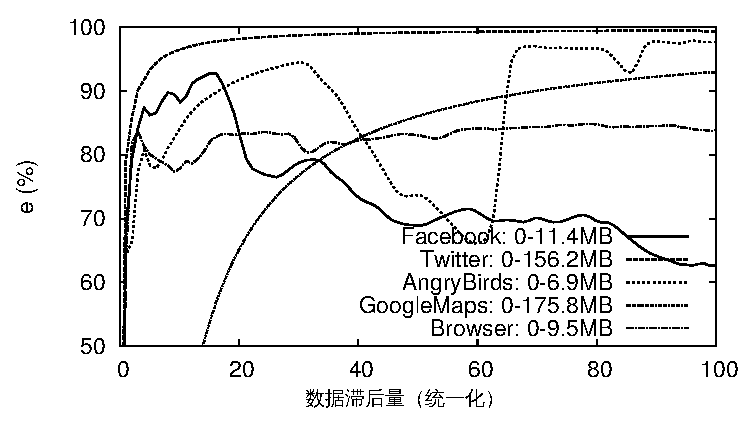
\includegraphics[width=0.9\columnwidth]{e-curve-app}
  \caption{不同形状的$e$曲线表明特定于应用的I/O模式。图中数据滞后量的范围统一到0至100,实际数值标记在应用名称旁。}
  \label{fig:e-curve-app}
\end{figure}

\textbf{原理5} 应用或用户特定的I/O访问模式需要动态的量化的策略设计,以在能耗和数据滞后量之间进行折衷和优化。

不同应用或用户的I/O访问模式差别很大。我们基于三个步骤来量化这种差异以及关键的权衡:(1)我们定义了适合我们上下文的数据滞后量指标。传统数据滞后量的定义或是基于时间~\cite{Ports:2010:TCA:1924943.1924963}或是基于版本~\cite{Bailis:2012:PBS:2212351.2212359},但是基于时间的定义很难与能量效率相联系,而常规文件系统中并没有对数据版本的严格定义。为此,我们定义了新的数据滞后量指标$s$为应用自上次生成检查点以来累计写操作的数据总量。如果应用在同一个地址上先后两次写了某个单位数据量,那么数据滞后量$s$增加两个单位量,而不是一个(在这个意义上,与传统基于版本的定义类似)。(2)基于上述原理3,我们定义能量效率比$e=o/s$,其中$o$是应用自上次生成检查点以来累计覆写的数据量。因为$o<s$,$e$的取值范围在$[0,1)$内。较大的$e$值意味着,对于相同的数据冲刷量,被覆写的数据较多,也就是节约的能耗较多。(3)基于上面两个定义,我们描绘$s$上的$e$曲线来表现增加数据滞后量带来的能量效率的变化。如图~\ref{fig:e-curve-app}所示,不同应用的$e$曲线呈现不同的形状,反映出对于不同应用最佳冲刷时间会有所不同(亦适用于不同用户)。理想状况下,应用的内存数据应该在$e$曲线达到峰值时进行冲刷,写入闪存。

\subsection{系统架构}

\begin{figure}
  \centering
  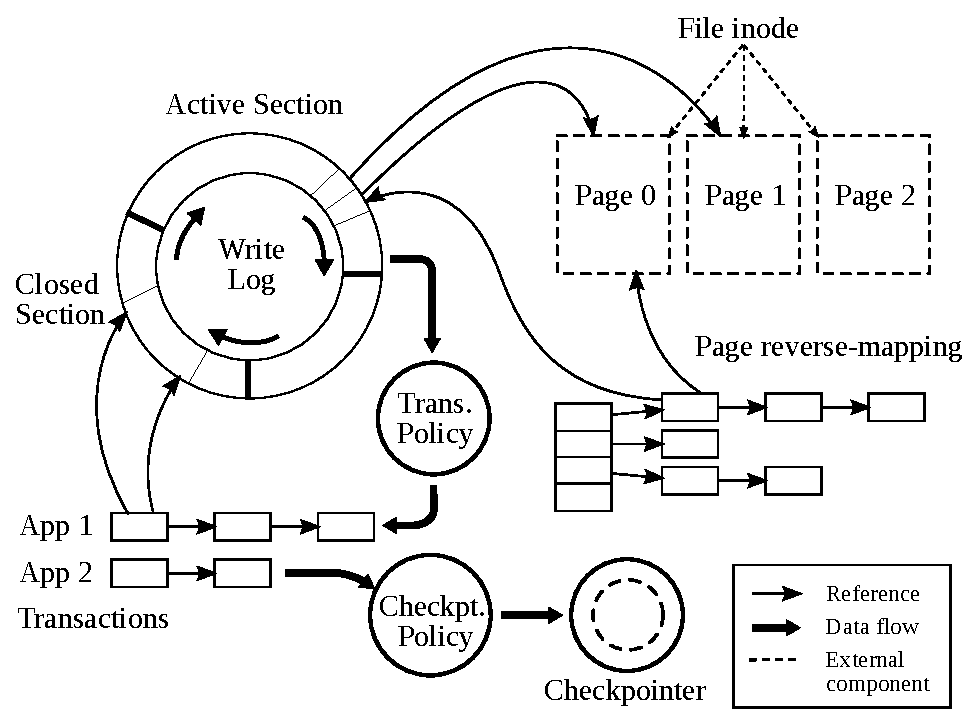
\includegraphics[width=0.8\columnwidth]{arch}
  \caption{MobiFS系统架构图}
  \label{fig:arch}
\end{figure}

MobiFS主要由五个模块构成:(1)页缓存,负责在内存中存储文件数据;(2)写日志,负责维护写操作的历史,由按序排列的许多记录项构成,每个记录项会引用一个页缓存中的物理页;(3)事务,写日志中的若干记录项归并为一组,它们的一致性不受覆写和重排序等优化的影响;(4)检查点生成器(checkpointer),负责调用底层闪存管理组件以原子性方式完成事务的持久化;(5)策略引擎,负责依据优化算法划分事务的边界,监听用户交互行为,并决定生成检查点的事务和时机。图~\ref{fig:arch} 描绘了MobiFS的系统架构。

MobiFS的设计充分考虑了与现有操作系统(Linux)的兼容和组件重用。它与操作系统共享现有的页缓存结构。对于页缓存的每个写操作,都会记入写日志,通常体现为在当前事务中(写日志的末尾)追加一个记录项,除非当前事务已经包含目标页地址的记录项。为此,我们需要维护一组从页地址到写日志项的逆向映射,以判断目标页地址是否已经存在于事务中。基于写日志和逆向映射,MobiFS建立起原子性事务机制。每个事务定义了可以进行覆写和重排序等优化的一个特定范围。最终,策略引擎指导检查点生成器保存事务到闪存,同时不影响用户交互。策略引擎根据每个手机应用甚至是用户的行为及其统计指标,做出动态的智能的判断。

在一个典型的配置中,不同手机应用会拥有自己独立的写日志和事务,但它们共享逆向映射、策略引擎和检查点生成器等组件。

\section{多版本缓冲事务技术}

在写日志中,可能同时引用逻辑上同一个缓冲页的多个物理版本。多版本缓冲事务用来管理这种关系。覆写和重排序等优化手段只允许用于单个多版本缓冲事务内部。由于检查点生成器可保证一个事务整体的持久化和原子性,这些优化不会导致闪存数据的任何不一致状态。

\subsection{写日志}

写日志是应用所有写操作按时间排列的历史记录。写日志包含两个段:活跃段(active section)处在写日志的末尾,新的记录项会被插入活跃段;闭合段(closed section)则包含准备生成检查点的记录项。 
 
在Android平台上,一份写日志的范围涵盖一个手机应用访问的所有目录。手机应用可能使用数据库SQLite保存数据,而SQLite是一个嵌入式数据库,它与每个应用捆绑的相关文件也需要托管给MobiFS,包含在应用的写日志范围内。
 
我们之所以能够面向特定应用进行写优化,一个重要原因在于手机应用的数据路径是静态的和相互隔离的,从而避免了应用间的一致性问题。当然,的确存在多个应用共享文件数据的情况,例如文件浏览器和相册应用可能同时管理照片存放的目录。这种情况下,相关应用需要在程序逻辑层面进行处理。即便不使用MobiFS,在现有Android的文件系统上,应用同样需要处理这类情况(例如,用户通过文件浏览器手动删除了相册中原本可见的照片)。 

\subsection{事务和版本}

一个多版本缓冲事务在其生命周期内经历三个状态:(1)当处于打开状态时,一个事务接收新的记录项,而这些记录项构成写日志中的活跃段。(2)当进入闭合状态时,该事务的所有记录项不再可以更改,转入写日志的闭合段。从打开状态到闭合状态的转换是单向的,不可逆的。(3)当进入提交状态时,该事务所有记录项对应的物理缓存页被检查点生成器原子性地刷出到闪存。成功提交之后,该事务及其记录项即从写日志中消除。 
 
当一个写操作到达时,MobiFS需要处理三种情况:(1)如果要写入的目标页不存在于逆向映射中,那么意味着写操作将进入一个未被写日志涵盖的页。MobiFS会在写日志中追加一个记录项,建立到缓存页的映射,并建立逆向映射。(2)如果逆向映射已经存在且指向一个写日志闭合段中的记录项,那么意味着写操作想要写入一个被保护的只读的事务。为此MobiFS对目标页执行写时拷贝(copy-on-write),并为新的页副本添加写日志记录项及映射/逆向映射。(3)如果逆向映射存在且指向一个写日志活跃段中的记录项(即打开的事务),那么意味着目标页不在被保护的闭合事务中,写操作可以直接更改目标页。

\subsection{故障复原}

多版本缓冲事务的边界不一定要和应用调用fsync()的时间对齐。在系统故障复原时,MobiFS依赖底层闪存管理组件,恢复已提交的事务或者回滚生成不完整检查点的事务。以我们基于日志文件系统Ext4组件的原型系统为例,它或者丢掉不完整的内部日志以回滚到之前的事务,或者重放日志内容恢复状态一致的事务。因此,文件系统或者数据库在系统复原后看到的数据总是对应于历史上某一个瞬间的状态。我们可以看到,MobiFS保证数据的一致性,而不保证严格意义上的已提交事务的持久性。

\subsection{检查点生成}

检查点生成器主要有两个职责。首先,它调用底层闪存管理组件保存事务数据。其次,当MobiFS载入时,检查所有分区并恢复一致的数据或回滚丢弃不一致的数据。很多现有文件系统(如Ext4和Btrfs)的闪存管理组件都可以很容易地进行重用。检查点生成器提供如下四个接口。 

\begin{itemize}
\item BEGIN\_TRANSACTION:在事务提交的开始调用,标志原子性保护的开端。 
\item SUBMIT\_ENTRY:在事务提交开始后,对该事务中每个写日志记录项调用。 
\item END\_TRANSACTION:在提交所有记录项后,即事务提交结束时,进行调用,标志原子性保护的结束。 
\item WAIT\_SYNC:支持非阻塞的调用方式,用于等待数据写入闪存。 
\end{itemize}

底层闪存管理组件需要保证在BEGIN\_TRANSACTION和END\_TRANSACTION调用之间写入的数据具有持久性和原子性。 

\section{优化策略和算法}

有两类策略在策略引擎中运行,事务划分策略和检查点生成策略。前者解决何时关闭一个事务的问题,后者解决何时将闭合事务写入闪存的问题。我们采用的通用规则是在手机处于空闲状态时(例如用户在阅读屏幕上的内容而没有操作行为的时候)生成检查点。我们的策略引擎设计为一个可扩展的框架,故有别于以下算法的其他具体策略亦可以使用。

\subsection{概述}

策略设计需要平衡多个相互冲突的目标:尽量少的数据滞后量,尽量高的能量效率和应用响应度。我们将三者的关系组织为一个可扩展的模块化的策略框架。 

MobiFS的策略框架包含三个模块:(1)事务划分模块,根据$e$曲线决定事务的边界,目标是获得尽量高的能量效率(\ref{subsec:point}节);该策略不依赖于有关用户操作分布的不现实的假设。(2)用户行为动态预测模块,根据预测结果可以推迟事务生成检查点的时间,目标是尽量不影响应用的响应度(\ref{subsec:interval}节)。(3)调度模块,协调多个应用的检查点生成过程(\ref{subsec:sched}节)。 
 
我们将能耗优化和响应度优化的策略独立分开,以避免复杂却又基于简化假设的多目标优化算法。我们的方式使得算法实现简洁而对实际系统有效。这里使用的很多技巧来源于我们大量第一手的优化经验。 

\subsection{事务划分算法}
\label{subsec:point}

\begin{figure}
\centering
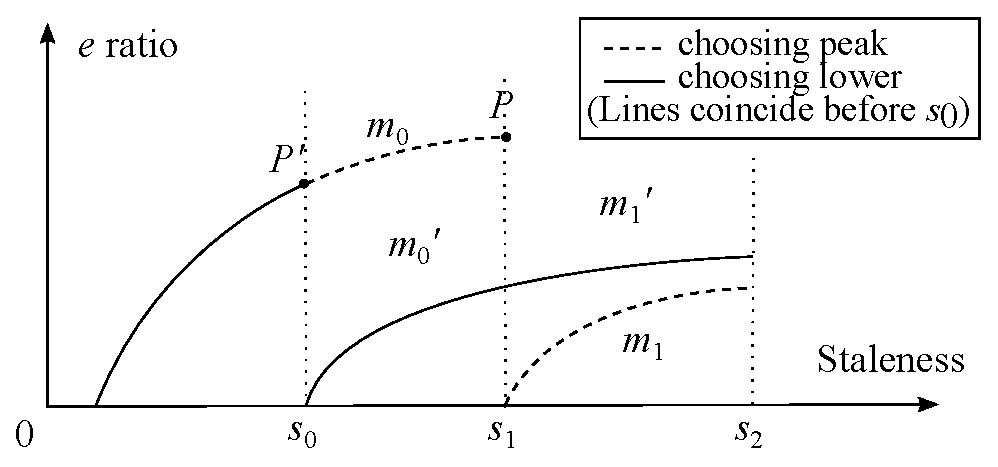
\includegraphics[width=0.7\columnwidth]{figures/tpl}
\caption{由选择不同的事务结束点产生的不同$e$曲线}
\label{fig:tpl}
\end{figure}

增加数据滞后量可以增加数据覆写的概率,从而节约数据冲刷量和相应的能耗,但付出的代价是更高的数据丢失的风险。所以我们面临这样的问题:MobiFS应该在多大程度上为减少能耗而增加数据滞后量?传统工作~\cite{Ma:2011:LPF:1989323.1989325, Mickens:2014:BFC:2616448.2616473, Ports:2010:TCA:1924943.1924963}仅通过设置一个较大的滞后量阈值来决定,而我们采用量化的动态的策略,依照每数据滞后量单元所节约的能耗量,即$e$比率(\ref{subsec:insight}节)来决定。直观来看,$e$曲线的顶点是最佳折衷点,因为对应的能耗节约率最高。我们的设计原则是减少数据丢失风险,除非有特定的原因不这样做(为提升能量效率等)。 

具体地,我们提出最佳折衷点定位算法(tradeoff point location,TPL),用于确定写日志中结束当前事务的记录项。每个来自应用的写操作都会增加数据滞后量,对应于$e$曲线上的一个点。当一个事务关闭时,$e$曲线重新从$e=0$开始计算,如图\ref{fig:tpl}所示。最理想地,结束事务的最佳点应当在$e$值最高的曲线顶点。我们采用反证法,假设另一个算法决定在$P'$点关闭当前事务,此时$x = s_0$,而曲线顶点$P$处于不同的位置$x = s_1$。那么我们可以在保持下一个事务结束点$x = s_2$不变的前提下,通过将当前事务结束点变为$P$来获得更多的能耗节约量。将当前事务结束点由$P'$变为$P$可以提高数据覆写发生的概率\footnote{注意这不是一个严格的数学证明。虽然可以构造出反例,但总体来说可能性更大。}。不失一般性,我们令$s_0 < s_1$;在$[s_0, s_1]$($[s_1, s_2]$)区段,我们算法的覆写数据量为$m_0$($m_1$),假设的算法的覆写数据量是$m_0'$($m_1'$)。那么我们有$m_0 - m_0' > m_1' -
m_1$,原因如下:区段$[s_0, s_1]$上,$e$曲线仍然在快速上升,表明可以覆写的数据量较大,但却被假设算法截断,会导致大量可以覆写的数据丧失覆写机会;相反地,由于$P$是曲线顶点,如果不被截断,曲线在$[s_1, s_2]$区段上是下降的,意味着较少的数据可以被覆写。上述公式简单等价变换可得$m_0 + m_1 > m_0' + m_1'$。综上,在$P$点截断曲线是限制数据滞后量的一种手段,而采用我们的策略可以尽可能多地增加数据覆写的可能。
 
在实际中,我们还需要应对其他一些挑战。曲线会出现波动导致算法定位在局部最优解,为此我们使用一个滑动窗口进行线性拟合来屏蔽这些波动。具体地,算法记录$e$曲线上过去$k$个点,拟合出一条曲线,然后根据其斜率判断是否到达顶点。我们之所以选择线性拟合,而不是更高阶的曲线拟合,是因为策略引擎对于每次写操作都要进行计算,算法复杂度会影响CPU的能耗。与此同时,我们设置了一个数据滞后量(或者冲刷间隔时间)的上限,以防止为等待顶点出现而无穷等待的情况。该算法的评测参见\ref{subsec:energy}节。

\subsection{行为间隔预测}
\label{subsec:interval}

\subsection{事务调度}
\label{subsec:sched}

\section{系统实现和效能评测}

\subsection{系统实现}

\subsection{评测方法}

\subsection{内存占用评测}
\label{subsec:eval-mem}

\subsection{应用和用户感知评测}

\subsection{应用响应度评测}

\subsection{能耗评测}
\label{subsec:energy}

\section{本章小结}

